\subsection{Separation properties}

\bd
A topological space $(M,\cO)$ is said to be \emph{T1}\index{topological space!T1 property} if for any two distinct points $p,q\in M$, $p\neq q$:
\bse
\exists \, U(p) \in \cO : q \notin U(p).
\ese
\ed

\bd
A topological space $(M,\cO)$ is said to be \emph{T2} or \emph{Hausdorff}\index{topological space!Hausdorff} if, for any two distinct points, there exist non-intersecting open neighbourhoods of these two points:
\bse
\forall \, p,q\in M : p\neq q \imp \exists \, U(p),V(q)\in \cO : U(p)\cap V(q) = \vn.
\ese
\ed

\be
The topological space $(\R^d,\cO_\mathrm{std})$ is T2 and hence also T1.
\ee

\be
The Zariski topology on an algebraic variety is T1 but not T2.
\ee

\be
The topological space $(M,\{\vn,M\})$ does not have the T1 property since for any $p \in M$, the only open neighbourhood of $p$ is $M$ and for any other $q\neq p$ we have $q\in M$. Moreover, since this space is not T1, it cannot be T2 either.
\ee

\br
There are many other ``T'' properties, including a \emph{T2\sfrac{1}{2}} property which differs from T2 in that the neighbourhoods are closed.
\er

\subsection{Compactness and paracompactness}

\bd
Let $(M,\cO)$ be a topological space. A set $C \se \cP(M)$ is called a \emph{cover}\index{cover}\index{topological space!(open) cover} (of $M$) if:
\bse
\bigcup C = M.
\ese
Additionally, it is said to an \emph{open} cover if $C \se \cO$.
\ed

\bd
Let $C$ be a cover. Then any subset $\widetilde{C}\se C$ such that $\widetilde{C}$ is still a cover, is called a \emph{subcover}. Additionally, it is said to be a \emph{finite} subcover if it is finite as a set.
\ed

\bd
A topological space $(M,\cO)$ is said to be \emph{compact}\index{compactness}\index{topological space!compact} if every open cover has a finite subcover.
\ed

\bd
Let $(M,\cO)$ be a topological space. A subset $N\se M$ is called \emph{compact} if the topological space $(N,\cO|_N)$ is compact.
\ed

Determining whether a set is compact or not is not an easy task. Fortunately though, for $\R^d$ equipped with the standard topology $\cO_\mathrm{std}$, the following theorem greatly simplifies matters.

\bt[Heine-Borel]\index{Heine-Borel theorem}
Let $\R^d$ be equipped with the standard topology $\cO_\mathrm{std}$. Then, a subset of $\R^d$ is compact if, and only if, it is closed and bounded.
\et

A subset $S$ of $\R^d$ is said to be \emph{bounded}\index{boundedness} if:
\bse
\exists \, r \in \R^+ : S \se B_r(0). 
\ese

\br
It is also possible to generalize this result to arbitrary metric spaces. A \emph{metric space}\index{metric space} is a pair $(M,d)$ where $M$ is a set and $d\cl M\times M \to \R$ is a map such that for any $x,y,z \in M$ the following conditions hold:
\ben
\item[i)] $d(x,y) \geq 0$;
\item[ii)] $d(x,y) = 0 \eqv x = y$;
\item[iii)] $d(x,y) = d(y,x) $;
\item[iv)] $d(x,y)\leq d(x,z)+d(y,z)$.
\een
A metric structure on a set $M$ induces a topology $\cO_d$ on $M$ by:
\bse
U \in \cO_d :\eqv \forall \, p \in U : \exists \, r \in \R^+ : B_r(p) \se U,
\ese
where the open ball in a metric space is defined as:
\bse
B_r(p) := \{x \in M \mid d(p,x) < r\}.
\ese
In this setting, one can prove that a subset $S\se M$ of a metric space $(M,d)$ is compact if, and only if, it is complete and totally bounded.
\er

\be
The interval $[0,1]$ is compact in $(\R,\cO_\mathrm{std})$. The one-element set containing $(-1,2)$ is a cover of $[0,1]$, but it is also a finite subcover and hence $[0,1]$ is compact from the definition. Alternatively, $[0,1]$ is clearly closed and bounded, and hence it is compact by the Heine-Borel theorem.
\ee

\be
The set $\R$ is not compact in $(\R,\cO_\mathrm{std})$. To prove this, it suffices to show that there exists a cover of $\R$ that does not have a finite subcover. To this end, let:
\bse
C := \{(n,n+1)\mid n \in \Z\} \cup \{(n+\tfrac{1}{2},n+\tfrac{3}{2})\mid n \in \Z\} .
\ese

This corresponds to the following picture.

\begin{figure}[h!]
\centering
\begin{tikzpicture}
\node (v2) at (4,0.5) {};
\node (v1) at (-4.75,0.5) {};
\draw  (v1) edge (v2);
\draw [-triangle 60] (v1) edge (v2);
\node (v3) at (-4.5,1) {};
\node (v4) at (3.5,1) {};
\draw  (v3) edge (v4);
\node (v5) at (-4.5,1.5) {};
\node (v6) at (3.5,1.5) {};
\draw  (v5) edge (v6);
\draw[fill=white]  (-0.5,1) circle (0.15);
\draw[fill=white]  (-3.5,1) node (v7) {} circle (0.15);
\draw[fill=white]  (2.5,1) circle (0.15);
\draw[fill=white]  (-2,1.5) circle (0.15);
\draw[fill=white]  (1,1.5) circle (0.15);
\draw  (-3.5,0.62) edge (-3.5,0.38);
\draw  (-2,0.62) edge (-2,0.38);
\draw  (-0.5,0.62) edge (-0.5,0.38);
\draw  (2.5,0.62) edge (2.5,0.38);
\draw  (1,0.62) edge (1,0.38);
\node at (-3.5,0) {$-1$};
\node at (-2,0) {$-\sfrac{1}{2}$};
\node at (-0.5,0) {$0$};
\node at (1,0) {$\sfrac{1}{2}$};
\node at (2.5,0) {$1$};
\node at (3.7,0) {$\R$};
\node at (-4.8,1.22) {$C\ \Bigl\{$};
\end{tikzpicture}
\end{figure}

It is clear that removing even one element from $C$ will cause $C$ to fail to be an open cover of $\R$. Therefore, there is no finite subcover of $C$ and hence, $\R$ is not compact.
\ee

\bt
Let $(M,\cO_M)$ and $(N,\cO_N)$ be compact topological spaces. Then $(M\times N,\cO_{M\times N})$ is a compact topological space.
\et

The above theorem easily extends to finite cartesian products. 

\bd
Let $(M,\cO)$ be a topological space and let $C$ be a cover. A \emph{refinement}\index{refinement} of $C$ is a cover $R$ such that:
\bse
\forall \, U \in R : \exists \, V \in C : U \se V .
\ese
\ed
Any subcover of a cover is a refinement of that cover, but the converse is not true in general. A refinement $R$ is said to be:
\bit
\item \emph{open} if $R\se \cO$;
\item \emph{locally finite} if for any $p\in M$ there exists a neighbourhood $U(p)$ such that the set:
\bse
\{U \in R \mid U \cap U(p) \neq \vn\}
\ese
is finite as a set.
\eit

Compactness is a very strong property. Hence often times it does not hold, but a weaker and still useful property, called paracompactness, may still hold.

\bd
A topological space $(M,\cO)$ is said to be \emph{paracompact}\index{topological space!paracompact}\index{paracompactness} if every open cover has an open refinement that is locally finite.
\ed

\bc
If a topological space is compact, then it is also paracompact.
\ec

\bd
A topological space $(M,\cO)$ is said to be \emph{metrisable} if there exists a metric $d$ such that the topology induced by $d$ is precisely $\cO$, i.e.\ $\cO_d=\cO$. 
\ed

\bt[Stone]
Every metrisable space is paracompact.
\et

\be
The space $(\R^d,\cO_\mathrm{std})$ is metrisable since $\cO_\mathrm{std}=\cO_d$ where $d = \|\cdot\|_2$. Hence it is paracompact by Stone's theorem.
\ee

\br
Paracompactness is, informally, a rather natural property since every example of a non-paracompact space looks artificial. One such example is the \emph{long line} (or \emph{Alexandroff line}). To construct it, we first observe that we could ``build'' $\R$ by taking the interval $[0,1)$ and stacking countably many copies of it one after the other. Hence, in a sense, $\R$ is equivalent to $\Z \times [0,1)$. The long line $L$ is defined analogously as $L:\omega_1\times [0,1)$, where $\omega_1$ is an uncountably infinite set. The resulting space $L$ is not paracompact.
\er

\bt
Let $(M,\cO_M)$ be a paracompact space and let $(N,\cO_N)$ be a compact space. Then $M\times N$ (equipped with the product topology) is paracompact.
\et

\bc
Let $(M,\cO_M)$ be a paracompact space and let $(N_i,\cO_{N_i})$ be compact spaces for every $1\leq i \leq n$. Then $M\times N_1\times\cdots\times N_n$ is paracompact.
\ec

\bd
Let $(M,\cO_M)$ be a topological space. A \emph{partition of unity}\index{partition of unity}  of $M$ is a set $\cF$ of continuous maps from $M$ to the interval $[0,1]$ such that for each $p\in M$ the following conditions hold:
\ben
\item[i)] there exists $U(p)$ such that the set $\{f \in \cF \mid \forall \, x \in U(p):f(x)\neq 0\}$ is finite;
\item[ii)] $\sum_{f\in \cF}f(p)=1$.
\een
If $C$ is an open cover, then $\cF$ is said to be \emph{subordinate} to the cover $C$ if:
\bse
\forall \, f \in \cF : \exists \, U \in C : f(x) \neq 0 \imp x \in U .
\ese
\ed

\bt
Let $(M,\cO_M)$ be a Hausdorff topological space. Then $(M,\cO_M)$ is paracompact if, and only if, every open cover admits a partition of unity subordinate to that cover.
\et

\be
Let $\R$ be equipped with the standard topology. Then $\R$ is paracompact by Stone's theorem. Hence, every open cover of $\R$ admits a partition of unity subordinate to that cover. As a simple example, consider $\cF = \{f,g\}$, where:
\bse
f(x) = \left\{ \ba{ll} 0 & \t{ if } x \leq 0\\ x^2 & \t{ if } 0\leq x\leq 1\\ 1 & \t{ if } x \geq 1 \ea \right.
\quad \t{and } \quad
g(x) = \left\{ \ba{ll} 1 & \t{ if } x \leq 0\\ 1-x^2 & \t{ if } 0\leq x\leq 1\\ 0 & \t{ if } x \geq 1 \ea \right. 
\ese
Then $\cF$ is a partition of unity of $\R$. Indeed, $f,g\cl \R \to [0,1]$ are both continuous, condition i) is satisfied since $\cF$ itself is finite, and we have $\forall \, x \in \R : f(x)+g(x)=1$.

Let $C:=\{(-\infty,1),(0,\infty)\}$. Then $C$ is an open cover of $\R$ and since:
\bse
f(x)\neq 0 \imp x \in (0,\infty) \quad \t{and} \quad g(x) \neq 0 \imp x \in (-\infty,1),
\ese
the partition of unity $\cF$ is subordinate to the open cover $C$.
\ee


\subsection{Connectedness and path-connectedness}

\bd
A topological space $(M,\cO)$ is said to be \emph{connected}\index{connectedness}\index{topological space!connected} unless there exist two non-empty, non-intersecting open sets $A$ and $B$ such that $M=A\cup B$.
\ed

\be
Consider $(\R\sm \{0\},\cO_\mathrm{std}|_{\R\sm\{0\}})$, i.e.\ $\R\sm\{0\}$ equipped with the subset topology inherited from $\R$. This topological space is not connected since $(-\infty,0)$ and $(0,\infty)$ are open, non-empty, non-intersecting sets such that $\R\sm\{0\}=(-\infty,0) \cup (0,\infty)$.
\ee

\bt
The interval $[0,1]\se\R$ equipped with the subset topology is connected.
\et

\bt
A topological space $(M,\cO)$ is connected if, and only if, the only subsets that are both open and closed are $\vn$ and $M$.
\et

\bq
\ben
\item[($\imp$)] Suppose, for the sake of contradiction, that there exists $U\se M$ such that $U$ is both open and closed and $U\notin\{\vn,M\}$. Consider the sets $U$ and $M\sm U$. Clearly, we have $U \cap M\sm U = \vn$. Moreover, $M\sm U$ is open since $U$ is closed. Therefore, $U$ and $M\sm U$ are two open, non-empty, non-intersecting sets such that $M = U \cup M \sm U$, contradicting the connectedness of $(M,\cO)$.
\item[($\Leftarrow$)] Suppose that $(M,\cO)$ is not connected. Then there exist open, non-empty, non-intersecting subsets $A,B\se M$ such that $M=A\cup B$. Clearly, $A \neq M$, otherwise we would have $B=\vn$. Moreover, since $B$ is open, $A=M\sm B$ is closed. Hence, $A$ is a set which is both open and closed and $A \notin \{\vn,M\}$.\qedhere
\een
\eq

\bd
A topological space $(M,\cO)$ is said to be \emph{path-connected}\index{path-connectedness}\index{topological space!path-connected} if for every pair of points $p,q\in M$ there exists a continuous curve $\g\cl[0,1]\to M$ such that $\g(0)=p$ and $\g(1)=q$.
\ed

\be
The space $(\R^d,\cO_\mathrm{std})$ is path-connected. Indeed, let $p,q\in\R^d$ and let:
\bse
\g(\l):=p+\l(q-p).
\ese
Then $\g$ is continuous and satisfies $\g(0)=p$ and $\g(1)=q$.
\ee

\be
Let $S:=\{(x,\sin(\tfrac{1}{x}))\mid x\in (0,1]\}\cup \{(0,0)\}$ be equipped with the subset topology inherited from $\R^2$.
\begin{center}
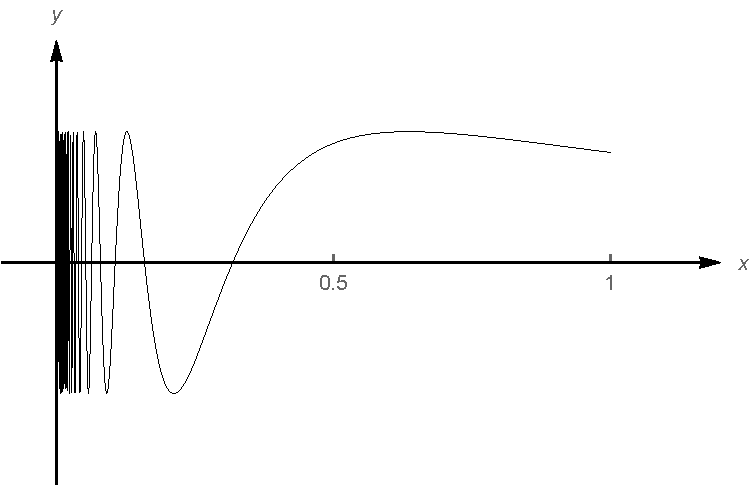
\includegraphics[scale=0.7]{graphics/sinoneoverx}
\end{center}
The space $(S,\cO_\mathrm{std}|_S)$ is connected but not path-connected.
\ee

\bt
If a topological space is path-connected, then it is also connected.
\et

\bq
Let $(M,\cO)$ be path-connected but not connected. Then there exist open, non-empty, non-intersecting subsets $A,B\subset M$ such that $M=A\cup B$. Let $p \in A$ and $q \in B$. Since $(M,\cO)$ is path-connected, there exists a continuous curve $\g\cl[0,1]\to M$ such that $\g(0)=p$ and $\g(1)=q$. Then:
\bse
[0,1] = \mathrm{preim}_\g(M) =  \mathrm{preim}_\g(A\cup B) =  \mathrm{preim}_\g(A)\cup  \mathrm{preim}_\g( B).
\ese
The sets $\mathrm{preim}_\g(A)$ and $ \mathrm{preim}_\g( B)$ are both open, non-empty and non-intersecting, contradicting the fact that $[0,1]$ is connected.
\eq

\subsection{Homotopic curves and the fundamental group}

\bd
Let $(M,\cO)$ be a topological space. Two curves $\g,\delta\cl[0,1]\to M$ such that:
\bse
\g(0)=\delta(0) \quad \t{and} \quad \g(1)=\delta(1)
\ese
are said to be \emph{homotopic}\index{homotopic curves} if there exists a continuous map $h \cl [0,1]\times[0,1]\to M$ such that for all $\l \in [0,1]$:
\bse
h(0,\l) = \g(\l) \quad \t{and} \quad h(1,\l)=\delta(\l).
\ese
\ed

Pictorially, two curves are homotopic if they can be continuously deformed into one another.

\begin{figure}[h!]
\centering
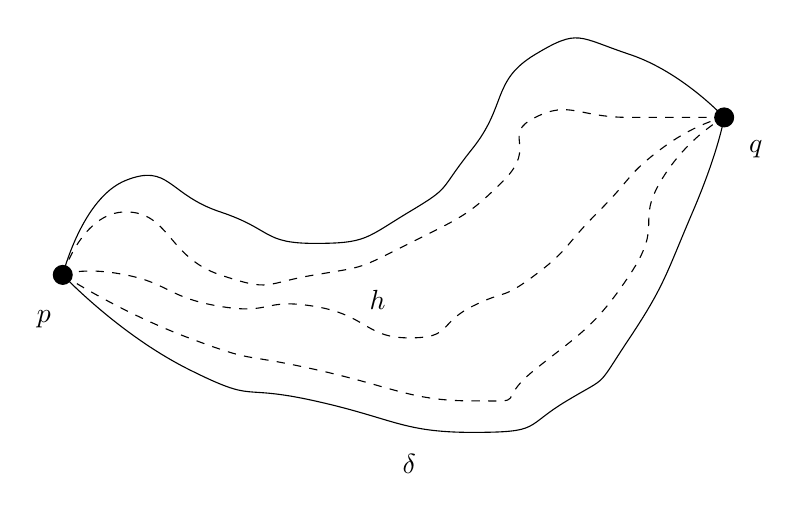
\begin{tikzpicture}[scale=0.8]

\draw  plot[smooth, tension=.999] coordinates {(-3,-0.5) (-2,1) (-0.5,0.5) (1,0) (2.5,0.5) (3.5,1.5) (4.5,3) (6,3) (7.5,2)};

\draw  plot[smooth, tension=.999] coordinates {(-3,-0.5) (-1,-2) (1,-2.5) (3.5,-3) (5,-2.5) (6,-1.5) (7,0.5) (7.5,2)};

\draw[dashed]  plot[smooth, tension=.999] coordinates {(-3,-0.5) (-2,0.5) (-0.5,-0.5) (1,-0.5) (2.5,0) (4,1) (4.5,2) (6,2) (7.5,2)};

\draw[dashed]  plot[smooth, tension=.999] coordinates {(-3,-0.5) (-2,-0.5) (-0.5,-1) (1,-1) (2.5,-1.5) (3.5,-1) (4.5,-0.5) (5.5,0.5) (6.5,1.5) (7.5,2)};

\draw[dashed]  plot[smooth, tension=.999] coordinates {(-3,-0.5) (-1,-1.5) (1,-2) (3.5,-2.5) (4.5,-2) (6,-0.5) (6.5,1) (7.5,2)};

\draw[fill=black]  (-3,-0.5) circle (0.15);
\draw[fill=black]  (7.5,2) circle (0.15);
\node at (-3.3,-1.2) {$p$};
\node at (8,1.5) {$q$};
\node at (-1.5,1.5) {$\g$};
\node at (2,-0.9) {$h$};
\node at (2.5,-3.5) {$\delta$};
\end{tikzpicture}
\end{figure}

\bp
Let $\g \sim \delta :\eqv$ ``$\g$ and $\delta$ are homotopic''. Then, $\sim$ is an equivalence relation.
\ep

\bd
Let $(M,\cO)$ be a topological space. Then, for every $p\in M$, we define the \emph{space of loops} at $p$ by:
\bse
\mathscr{L}_p := \{\g\cl[0,1]\to M \mid \g \t{ is continuous and } \g(0)=\g(1)\}.
\ese
\ed

\bd
Let $\mathscr{L}_p$ be the space of loops at $p\in M$. We define the \emph{concatenation} operation $*\cl \mathscr{L}_p\times\mathscr{L}_p\to\mathscr{L}_p$ by:
\bse
(\g * \delta) (\l):= \left\{ \ba{ll} \g(2\l) & \t{if } 0\leq \l \leq \tfrac{1}{2}\\ \delta(2\l-1) & \t{if } \tfrac{1}{2}\leq \l \leq 1 \ea \right.
\ese
\ed

\bd
Let $(M,\cO)$ be a topological space. The \emph{fundamental group}\index{fundamental group} $\pi_1(p)$\index{$\pi_1(p)$} of $(M,\cO)$ at $p\in M$ is the set:
\bse
\pi_1(p) := \mathscr{L}_p/\!\sim\ = \{[\g] \mid \g \in \mathscr{L}_p\},
\ese
where $\sim$ is the homotopy equivalence relation, together with the map 
\bi{rrCl}
\bullet \cl & \pi_1(p)\times \pi_1(p) &\to &\pi_1(p)\\
&(\g,\delta)&\mapsto & [\g]\bullet[\delta]:=[\g*\delta] .
\ei
\ed

\br
Recall that a group\index{group} is a pair $(G,\bullet)$ where $G$ is a set and $\bullet \cl G\times G \to G$ is a map (also called \emph{binary operation}) such that:
\ben
\item[i)] $\forall \, a,b,c \in G : (a\bullet b)\bullet c = a \bullet (b\bullet c)$;
\item[ii)] $\exists \, e \in G : \forall \, g \in G : g \bullet e = e \bullet g = g$;
\item[iii)] $\forall \, g \in G : \exists \, g^{-1}\in G: g \bullet g^{-1} = g^{-1} \bullet g = e$.
\een
A group is called \emph{abelian (or commutative)} if, in addition, $a\bullet b = b \bullet a$ for all $a,b\in G$.

A \emph{group isomorphism}\index{isomorphism!of groups} between two groups $(G,\bullet)$ and $(H,\circ)$ is a bijection $\phi\cl G \to H$ such that:
\bse
\forall \, a,b \in G:\phi(a \bullet b) = \phi(a)\circ\phi(b).
\ese
If there exists a group isomorphism between $(G,\bullet)$ and $(H,\circ)$, we say that $G$ and $H$ are (group theoretic) isomorphic and we write $G \cong_\mathrm{grp} H$.
\er

The operation $\bullet$ is associative (since concatenation is associative); the neutral element of the fundamental group $(\pi_1(p),\bullet)$ is (the equivalence class of) the constant curve $\g_e$ defined by:
\bi{rrCl}
\g_e \cl & [0,1] & \to & M\\
& \l & \mapsto & \g_e(0) = p
\ei
Finally, for each $[\g]\in\pi_1(p)$, the inverse under $\bullet$ is the element $[-\g]$, where $-\g$ is defined by:
\bi{rrCl}
-\g \cl & [0,1] & \to & M\\
& \l & \mapsto & \g(1-\l)
\ei

All the previously discussed topological properties are ``boolean-valued'', i.e.\ a topological space is either Hausdorff or not Hausdorff, either connected or not connected, and so on. The fundamental group is a ``group-valued'' property, i.e.\ the value of the property is not ``either yes or no'', but a group. 

A property of a topological space is called an \emph{invariant} if any two homeomorphic spaces share the property. A \emph{classification} of topological spaces would be a list of topological invariants such that any two spaces which share these invariants are homeomorphic. As of now, no such list is known. 

\be
The 2-sphere is defined as the set:
\bse
S^2:=\{(x,y,z)\in \R^3\mid x^2+y^2+z^2=1\}
\ese
equipped with the subset topology inherited from $\R^3$.

\begin{center}
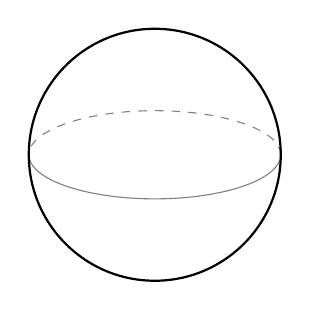
\begin{tikzpicture}[scale=0.8]
  \draw[gray,dashed] (2,0) arc (0:180:2cm and 0.7cm);
  \draw[gray] (2,0) arc (0:-180:2cm and 0.7cm);
  \draw[thick] (0,0) circle[radius=2cm];
\end{tikzpicture}
\end{center}

The sphere has the property that all the loops at any point are homotopic, hence the fundamental group (at every point) of the sphere is the trivial group:
\bse
\forall \, p \in S^2 : \pi_1(p) = 1:=\{[\g_e]\}.
\ese
\ee

\be
The cylinder is defined as $C:=\R\times S^1$ equipped with the product topology.

\begin{center}
\begin{tikzpicture}
  \draw[dashed] (-3.75,0) -- (-3,0);
  \draw[dashed] (3,0) -- (3.75,0);
  \draw[dashed] (-3.5,-1.5) -- (3.5,-1.5);
  \draw[dashed] (-3.75,-3) -- (-3,-3);
  \draw[dashed] (3,-3) -- (3.75,-3);
  \draw[thick] (-3,0) -- (3,0);
  \draw[thick] (-3,-3) -- (3,-3);
  \draw[dashed,gray] (0,0) arc (90:-90:0.75cm and 1.5cm);
  \draw[gray] (0,0) arc (90:270:0.75cm and 1.5cm);
\end{tikzpicture}
\end{center}

A loop in $C$ can either go around the cylinder (i.e.\ around its central axis) or not. If it does not, then it can be continuously deformed to a point (the identity loop). If it does, then it cannot be deformed to the identity loop (intuitively because the cylinder is infinitely long) and hence it is a homotopically different loop. The number of times a loop winds around the cylinder is called the \emph{winding number}\index{winding number}. Loops with different winding numbers are not homotopic.

Moreover, loops with different \emph{orientations} are also not homotopic and hence we have:
\bse
\forall \, p \in C : (\pi_1(p),\bullet) \cong_\mathrm{grp}(\Z,+).
\ese
\ee

\be
The 2-torus is defined as the set $T^2:=S^1\times S^1$ equipped with the product topology.
\begin{center}
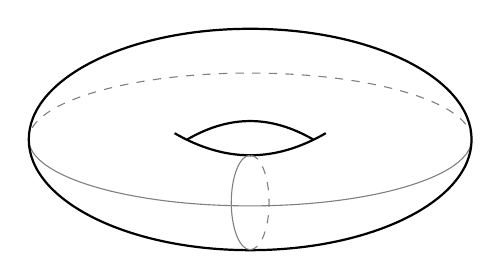
\begin{tikzpicture}[scale=0.8]
  \draw[thick] (-1,0) to[bend left] (1,0);
  \draw[thick] (-1.2,.1) to[bend right] (1.2,.1);
  \draw[gray] (100pt,0) arc (0:-180:100pt and 30pt);
  \draw[gray,dashed] (100pt,0) arc (0:180:100pt and 30pt);
  \draw[thick] (0,0) ellipse (100pt and 50pt);
  \draw[gray,dashed]  (0,-1.75) arc (-90:90:0.3 and 0.75);
  \draw[gray] (0,-1.75) arc (-90:-270:0.3 and 0.75);
  \end{tikzpicture}
\end{center}
A loop in $T^2$ can intuitively wind around the cylinder-like part of the torus as well as around the hole of the torus. That is, there are two independent winding numbers and hence:
\bse
\forall \, p \in T^2 : \pi_1(p) \cong_\mathrm{grp}\Z\times \Z,
\ese
where $\Z\times \Z$ is understood as a group under pairwise addition.
\ee







































